\documentclass[10pt,a4paper]{article}
\usepackage[T1]{fontenc}
\usepackage[utf8]{inputenc}
\usepackage{lmodern}
\usepackage[margin=2cm]{geometry}
\usepackage{graphicx}
\usepackage{xcolor}
\usepackage{booktabs}
\usepackage{enumitem}
\usepackage{parskip}
\usepackage{float}
\usepackage{tikz}
\usetikzlibrary{positioning,arrows.meta,fit}
\usepackage[colorlinks=true,linkcolor=black,urlcolor=teal]{hyperref}

% Charts come from ../results/, screenshots from docs/img/. Compile from inside docs/.
\graphicspath{{../results/}{img/}}
\setlist{itemsep=2pt,topsep=4pt}
\newcommand{\code}[1]{\texttt{#1}}

\title{\textbf{Community Status Network}\\[4pt]
\large A fault-tolerant distributed service for live community status reports\\[2pt]
\normalsize Distributed Systems project (BSE 4103 / BCS 3107)}
% Swap these two lines' roles in the Contributions section if the split of work was different.
\newcommand{\memberA}{Woduwa Marvin Wamoni}
\newcommand{\memberB}{Nyomore Henry}
\author{Woduwa Marvin Wamoni\\\small 23/2/370/W/605 \and Nyomore Henry\\\small 23/2/370/W/736}
\date{November 2026}

\begin{document}
\maketitle

\begin{abstract}
\noindent The Community Status Network lets residents report local problems (power cuts, dry
water points, blocked roads), lets moderators verify and resolve them, and shows every change to
all viewers as it happens. Three cooperating server processes each hold a full copy of the data.
One leader orders the changes, and a change is acknowledged only after a majority has written it
to disk, so the service survives the loss of any one server without losing an acknowledged change.
It is written with the Python~3 standard library only.
\end{abstract}

%======================================================================
\section{(a) Requirements and architecture}

\subsection{Users}

\begin{description}[leftmargin=2.4cm,style=sameline]
\item[Resident] Submits a report and may edit its description.
\item[Moderator] Does what a resident does and may also set a report to \emph{verified} or
\emph{resolved}.
\item[Viewer] Watches the list of reports, which updates live without refreshing.
\end{description}

\subsection{Functional requirements}

\begin{enumerate}[label=\textbf{FR\arabic*}]
\item A resident can submit a report with a type (power, water, road, other), a location and a
description.
\item Any user can retrieve reports from any server, filtered by type, status or location, and
can see the full change history of one report.
\item A report can be updated; two conflicting updates to the same report must never both
succeed.
\item Every change is pushed to connected viewers in real time.
\item The service keeps working when one server fails.
\item A restarted server recovers its data from its own log and catches up on what it missed.
\end{enumerate}

Non-functional constraints: Python standard library only, three server processes, no
acknowledged write may be lost when a single server fails.

\subsection{Distributed processes}

\begin{itemize}
\item \textbf{Three server processes} (nodes N1, N2, N3). Each has an API layer, a coordinator
(locks and version checks), an in-memory store and a write-ahead log (WAL) file. One node is the
\emph{leader}; the others are \emph{followers}.
\item \textbf{Client processes:} the web application in a browser, the command-line client, and
the live-feed viewer. Any number may run at once.
\end{itemize}

\subsection{Hardware and software components}

\begin{tabular}{@{}p{0.27\textwidth}p{0.68\textwidth}@{}}
\toprule
Component & Description \\
\midrule
Hardware & One laptop running three processes on ports 8001--8003, or three laptops on one
local network. Phones and laptops act as clients. One disk file per node holds its log. \\
Server software & \code{csn/server.py} (HTTP server), \code{csn/store.py} (store and
coordinator), \code{csn/wal.py} (log), \code{csn/node.py} (replication, heartbeats, election,
catch-up), \code{csn/feed.py} (live feed). \\
Client software & \code{web/live.html} (web application), \code{csn/client.py} (client library
with timeout, retry and failover), \code{csn/cli.py} (command line). \\
Configuration & \code{config.json} lists the address of each node. \\
\bottomrule
\end{tabular}

\subsection{Communication links}

\begin{description}[leftmargin=1.2cm,style=sameline]
\item[A] Client to node: HTTP/REST with JSON bodies, plus Server-Sent Events (one long-lived HTTP
response) for the live feed.
\item[B] Leader to followers: an HTTP POST for each change (replication), and an HTTP GET by
which a node fetches log entries it is missing (catch-up).
\item[C] Node to node: an HTTP POST heartbeat every second, carrying the sender's identity, its
current leader, its term number and the length of its log. The same messages drive leader
election.
\end{description}

\subsection{Architecture diagram}

\begin{figure}[H]
\centering
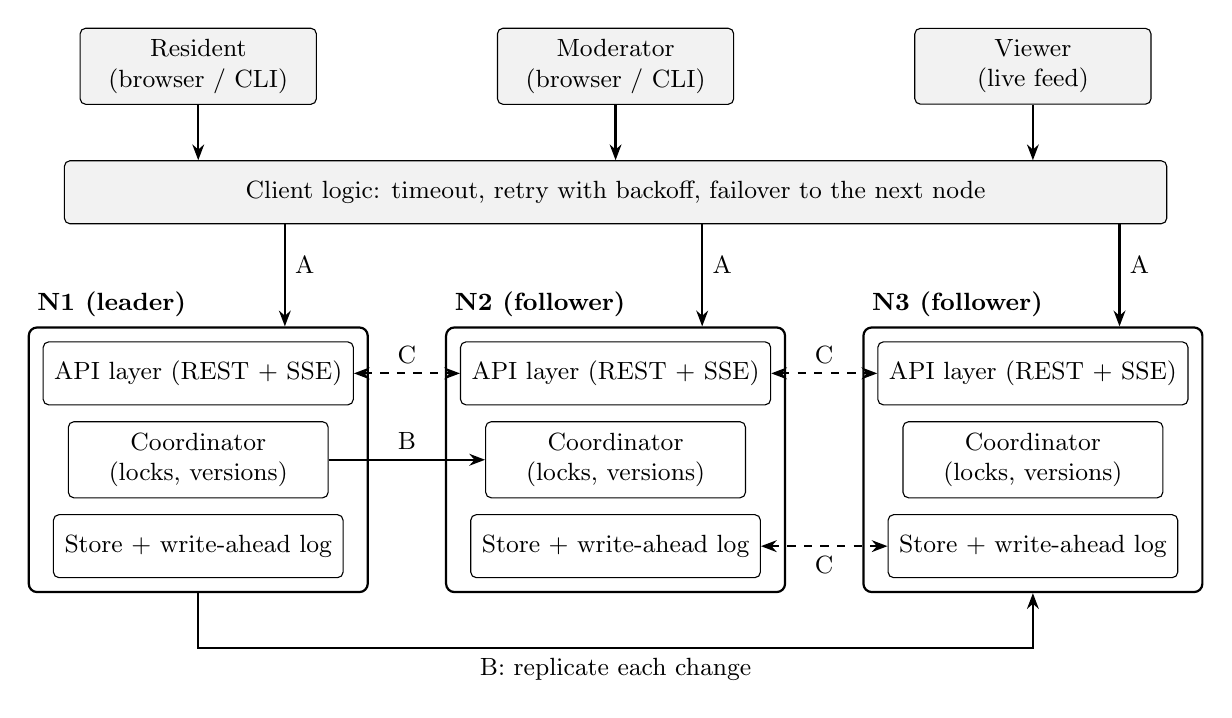
\begin{tikzpicture}[
  font=\small,
  box/.style={draw, rounded corners=2pt, align=center, minimum height=8mm, inner sep=4pt},
  client/.style={box, fill=gray!10, minimum width=30mm},
  layer/.style={box, fill=white, minimum width=33mm},
  link/.style={-{Stealth[length=2mm]}, thick},
  both/.style={{Stealth[length=2mm]}-{Stealth[length=2mm]}, thick, dashed}
]
% clients
\node[client] (res) at (-5.3,6.2) {Resident\\(browser / CLI)};
\node[client] (mod) at (0,6.2) {Moderator\\(browser / CLI)};
\node[client] (view) at (5.3,6.2) {Viewer\\(live feed)};
\node[box, fill=gray!10, minimum width=140mm] (lib) at (0,4.6)
  {Client logic: timeout, retry with backoff, failover to the next node};
\draw[link] (res) -- (res |- lib.north);
\draw[link] (mod) -- (mod |- lib.north);
\draw[link] (view) -- (view |- lib.north);

% nodes
\foreach \x/\nid/\nrole in {-5.3/N1/leader, 0/N2/follower, 5.3/N3/follower} {
  \node[layer] (api\nid) at (\x,2.3) {API layer (REST + SSE)};
  \node[layer, below=2mm of api\nid] (co\nid) {Coordinator\\(locks, versions)};
  \node[layer, below=2mm of co\nid] (st\nid) {Store + write-ahead log};
  \node[draw, thick, rounded corners=3pt, fit=(api\nid)(co\nid)(st\nid), inner sep=5pt,
        label={[font=\small\bfseries, anchor=south west]north west:{\nid{} (\nrole)}}] (node\nid) {};
  \draw[link] ([xshift=11mm]node\nid.north |- lib.south) -- node[right, pos=0.4]{A} ([xshift=11mm]node\nid.north);
}

% replication and heartbeat
\draw[link] (coN1.east) -- node[above]{B} (coN2.west);
\draw[link] (nodeN1.south) -- ++(0,-0.7) -| node[below, pos=0.25]{B: replicate each change} (nodeN3.south);
\draw[both] (apiN1.east) -- node[above]{C} (apiN2.west);
\draw[both] (apiN2.east) -- node[above]{C} (apiN3.west);
\draw[both] (stN2.east) -- node[below]{C} (stN3.west);
\end{tikzpicture}
\caption{Architecture. A: client to node (HTTP/REST/JSON and Server-Sent Events). B: leader to
followers (replication of each change). C: node to node (heartbeats and leader election, dashed).}
\label{fig:arch}
\end{figure}

\paragraph{Explanation.} A client may contact any node. Reads are answered from that node's own
copy. A write that arrives at a follower is forwarded to the leader, and the leader's answer is
relayed back unchanged. Inside the leader, the coordinator checks the write under a lock, the
store appends it to the WAL and applies it to memory, and the node replicates it to the followers
over link~B. Each follower appends the same entry to its own WAL and applies it. All nodes
exchange heartbeats over link~C; these detect a dead node and select a new leader. The client
logic at the top is what lets a user keep working when the node they were talking to disappears.

\paragraph{Data model.} A \emph{report} has \code{id}, \code{type}, \code{location},
\code{description}, \code{status}, \code{version}, \code{updated\_by} and \code{updated\_at}. A
\emph{log entry} has \code{seq} (its position in the log), \code{op} (create or update), the
complete resulting report as \code{payload}, and the \code{node\_id} that produced it. Because
each entry stores the whole report, the log is also the history of every report.

%======================================================================
\section{(b) Implementation}

\subsection{A working prototype with communicating processes}

The prototype consists of three server processes and any number of client processes. A node is
started with \code{python3 -m csn.server -{}-id N1}; \code{python3 demo.py} starts all three and
runs a narrated walkthrough. The servers use \code{http.server} with one thread per connection;
clients use \code{http.client} (Python) or \code{fetch} and \code{EventSource} (browser). No
third-party package is used.

\subsection{Communication mechanism: HTTP/REST with JSON}

\begin{table}[H]
\centering\small
\begin{tabular}{@{}lp{0.55\textwidth}@{}}
\toprule
Request & Purpose \\
\midrule
\code{POST /reports} & Submit a report. Returns 201 and the report. \\
\code{GET /reports?type=\&status=\&location=} & List or filter reports (any node). \\
\code{GET /reports/<id>} & One report. \\
\code{GET /reports/<id>/history} & Every version of one report, from the WAL. \\
\code{PATCH /reports/<id>} & Update; must include \code{base\_version}. 409 if stale. \\
\code{GET /events} & Live feed (Server-Sent Events); resumable by event id. \\
\code{GET /health}, \code{GET /nodes} & Node state and node addresses. \\
\code{POST /internal/replicate} & Leader to follower: one log entry (link B). \\
\code{POST /internal/heartbeat} & Node to node (link C). \\
\code{GET /internal/log?after=N} & Entries after position N (catch-up). \\
\bottomrule
\end{tabular}
\caption{The interface. Status codes: 400 invalid input, 404 unknown report, 409 version
conflict, 413 body too large, 503 no leader or no majority.}
\end{table}

\subsection{How data is exchanged}

A resident submits a report by sending JSON to any node:
\begin{verbatim}
POST /reports
{"type": "water", "location": "Kira", "description": "Borehole dry",
 "updated_by": "alice", "request_id": "3f9a..."}

201 Created
{"id": "R1", "type": "water", "location": "Kira",
 "description": "Borehole dry", "status": "open", "version": 1,
 "updated_by": "alice", "updated_at": 1794381234.5}
\end{verbatim}

A moderator verifies it, stating the version they read:
\begin{verbatim}
PATCH /reports/R1
{"updated_by": "grace", "role": "moderator",
 "base_version": 1, "status": "verified"}

200 OK      {"id": "R1", ... "status": "verified", "version": 2, ...}
\end{verbatim}

Every connected viewer then receives this event on its open \code{/events} stream, whichever node
it is connected to:
\begin{verbatim}
id: 2
event: report
data: {"seq": 2, "op": "updated", "report": {...},
       "served_by": "N3"}
\end{verbatim}

Between nodes, the leader posts the log entry, its term and its name to
\code{/internal/replicate}, and the follower answers \code{\{"ack": true, "last\_seq": 2\}}.

\subsection{Storage and clients}

Each node keeps a write-ahead log, one JSON line per change. The rule is \emph{log first, then
memory, then acknowledge}: an entry is forced to disk (\code{fsync}) before it is applied or
confirmed, and a restarted node rebuilds its memory by replaying the file. The web application
(\code{web/live.html}, one file, no build step) and the command-line client offer the same
operations and share the same client logic: a timeout on every request, retries with exponential
backoff, and failover to the next node.

%======================================================================
\section{(c) Coordination and consistency}

\subsection{One writer orders all changes}

Only the leader accepts writes; followers forward them. All changes therefore pass through one
place that assigns them consecutive log positions, and every node applies them in the same order.

\subsection{Locking strategy}

The leader holds \textbf{one lock per report}. An update takes the lock of the report it changes,
so two edits to the \emph{same} report run one after the other, while edits to \emph{different}
reports run in parallel. New reports share a single creation lock so that report numbers and log
order stay consistent. Locks are always taken in the same order, which rules out deadlock.

\subsection{Preventing conflicting updates: optimistic version checks}

Every report has a \code{version}. A client must send \code{base\_version}, the version it last
read. Under the report's lock the leader compares the two:

\begin{itemize}
\item If they are equal, the update is applied, the version increases by one, the entry is logged
and replicated, and the client receives 200.
\item If they differ, somebody else changed the report first. Nothing is written and the client
receives \textbf{409 Conflict} together with the current report.
\end{itemize}

Because the comparison and the write happen under the same lock, two updates based on the same
version can never both succeed. This prevents the ``lost update'' problem.

\paragraph{Resolving a conflict.} The loser is told, not silently overwritten. In the web
application a dialog shows the latest version beside the user's unsaved edit and offers two
choices: apply the edit on top of the latest version (a new request with the new
\code{base\_version}) or discard it.

\paragraph{Evidence.} Automated tests start two threads that edit the same report from the same
version and assert exactly one 200 and one 409; a second test does the same with ten threads and
asserts exactly one winner; a third confirms that edits to different reports do not block each
other. Under load, 2.5\% to 3.7\% of all requests were 409 responses (Section~\ref{sec:perf}),
and after every run the three nodes held identical data.

\subsection{Keeping the copies consistent: majority replication}

The leader acknowledges a write only when it and at least one follower (two of three) have stored
the entry; the third follower completes in the background.

\begin{itemize}
\item Waiting for \emph{all} followers would stop all writes whenever one node is down.
\item Not waiting at all would be fastest but could lose acknowledged writes if the leader died.
\item Waiting for a majority costs one network round trip per write and guarantees that an
acknowledged write survives the loss of any one node.
\end{itemize}

Followers apply entries strictly in log order. If entry $n+1$ arrives before entry $n$, the
follower waits briefly for the gap to fill. A test with concurrent writers confirms that the
three log files end up identical.

\subsection{Other consistency points}

\begin{itemize}
\item \textbf{Reads} are served from the local copy of the node asked. The follower outside the
majority may lag by milliseconds, so a read there can briefly miss a write that was just
acknowledged. This is a deliberate trade of freshness for availability and speed.
\item \textbf{Retried submits.} A client attaches a \code{request\_id} to each submit. If a retry
arrives for a submit that was already applied, the leader returns the existing report instead of
creating a duplicate.
\end{itemize}

%======================================================================
\section{(d) Fault handling and reliability}

\subsection{Failure detection and leader election}

Nodes exchange heartbeats every second. A peer silent for three seconds is considered dead. If
the leader is dead, each live node selects the live node with the lowest identifier as the new
leader. Each election increases a \emph{term} number carried in heartbeats and replication
messages; nodes follow the highest term, and followers refuse replication from a leader with an
old term. Before accepting writes, a new leader first fetches any entries it is missing from the
other live node, so no acknowledged write is dropped.

\subsection{Failure scenarios demonstrated}

\paragraph{1. The leader is killed under load.} The leader process was killed with
\code{SIGKILL} while clients were writing (Table~\ref{tab:fail}). A new leader was elected in
3.3~s. Writes were unavailable for 3.3~s; reads never failed. A user write issued during the
outage completed after 3.4 to 5.1~s (mean 4.0~s) through client retries, without the user doing
anything. None of the 3,982 acknowledged writes was lost.

\paragraph{2. A server restarts.} The killed node was started again. It replayed its WAL, asked
its peers who the leader was, joined as a follower and fetched the entries it had missed. It was
serving requests after 0.08~s and had caught up (963 to 1,202 entries) after 0.13~s. A returning
former leader does not reclaim leadership. If its log contains a write that was never
acknowledged and disagrees with the new leader's log, it sets its log aside and downloads the
leader's.

\paragraph{3. A dropped connection to a viewer.} When the node serving a live feed dies, the
viewer connects to the next node and sends the id of the last event it received; the new node
replays everything after it. In the browser this was verified by killing the node serving the
page: the page reported that it had reconnected through another node and that one update had been
replayed.

\paragraph{4. Timeouts and unavailable service.} Every client request has a timeout (5~s in the
library). On a network error or a 502/503/504 answer, the client retries up to eight times with
exponential backoff (0.25~s, 0.5~s, 1~s, 2~s, \dots) and random jitter, moving to the next node
each time. Answers 400, 404 and 409 are real answers and are not retried.

\paragraph{5. No majority.} With two of three nodes down, the survivor answers writes with 503
and continues to serve reads. The web application states this in words.

\begin{table}[H]
\centering
\begin{tabular}{@{}rrrrrrr@{}}
\toprule
Trial & Election & Write outage & User write & Lost acked & Restart: & Restart: \\
 & (s) & (s) & latency (s) & writes & serving (s) & caught up (s) \\
\midrule
1 & 3.35 & 3.35 & 3.40 & 0 of 1304 & 0.08 & 0.13 \\
2 & 3.31 & 3.30 & 5.07 & 0 of 1380 & 0.07 & 0.13 \\
3 & 3.30 & 3.35 & 3.43 & 0 of 1298 & 0.08 & 0.13 \\
\midrule
Mean & 3.32 & 3.33 & 3.97 & & 0.08 & 0.13 \\
\bottomrule
\end{tabular}
\caption{Leader killed under load, then restarted (heartbeat 1~s, dead after 3~s), measured on
11 November 2026. Read failures: 0 in every trial. The three WAL files were identical after every
trial.}
\label{tab:fail}
\end{table}

\subsection{The same failure seen in the web application}

The failover was also recorded in a browser connected to follower N3, with timings taken by the
script that drove the browser (Table~\ref{tab:browser}, Figure~\ref{fig:browser}). This run had
no background load, so it shows what one user experiences.

\begin{table}[H]
\centering\small
\begin{tabular}{@{}lr@{}}
\toprule
Event & Time \\
\midrule
Leader N1 killed (\code{SIGKILL}) & 0.00 s \\
N2 reports itself as the new leader & 2.74 s \\
Report submitted in the browser at the kill is saved (5 retries) & 5.17 s \\
\midrule
N1 restarted: answering requests & 0.09 s after start \\
N1 restarted: caught up on 4 missed entries, as a follower & 0.09 s after start \\
\midrule
Node serving the page (N3) killed: live feed back through N1 & 0.53 s \\
\bottomrule
\end{tabular}
\caption{Timings of one failover observed from the browser, 11 November 2026.}
\label{tab:browser}
\end{table}

Two of these figures need explaining. The election took 2.74~s, less than the 3.3~s in
Table~\ref{tab:fail}, because the three-second timeout counts from the \emph{last heartbeat
received}, which can be up to one second before the kill. The browser's write took 5.17~s although
a leader existed after 2.74~s, because retries follow a fixed backoff schedule (roughly 0.25, 0.5,
1, 2, 2~s): the attempt just before the election finished failed, and the next one was two
seconds later. A shorter maximum backoff would reduce this at the cost of more requests during
an outage.

\begin{figure}[H]
\centering
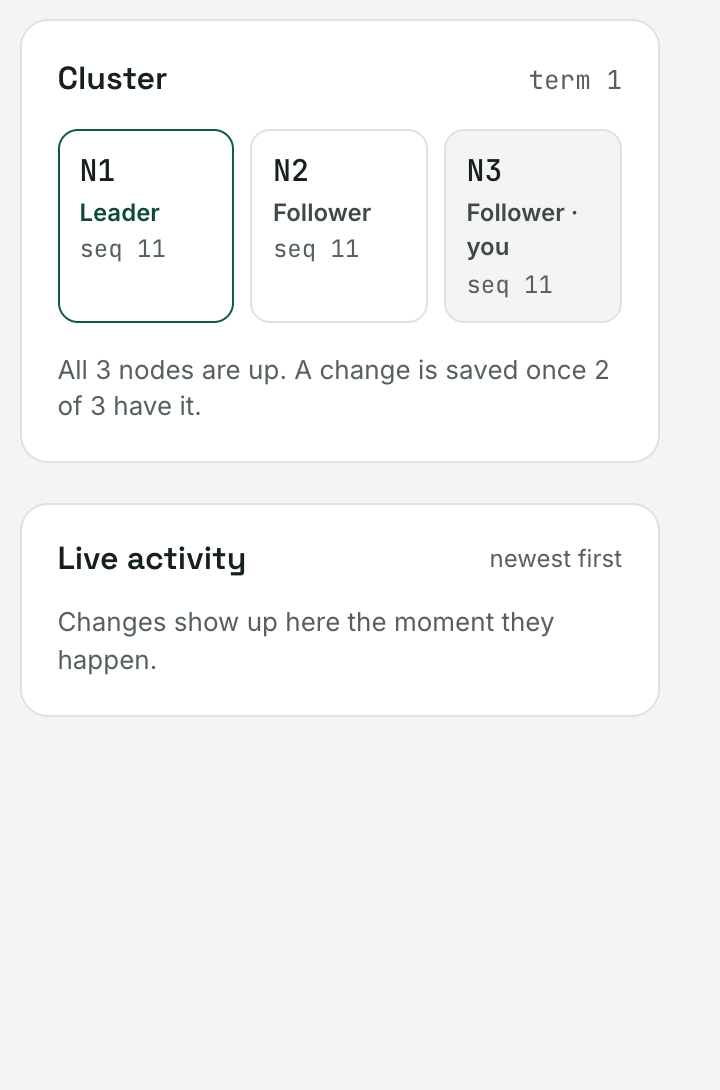
\includegraphics[width=0.24\textwidth]{failover-1-before-cluster.png}\hfill
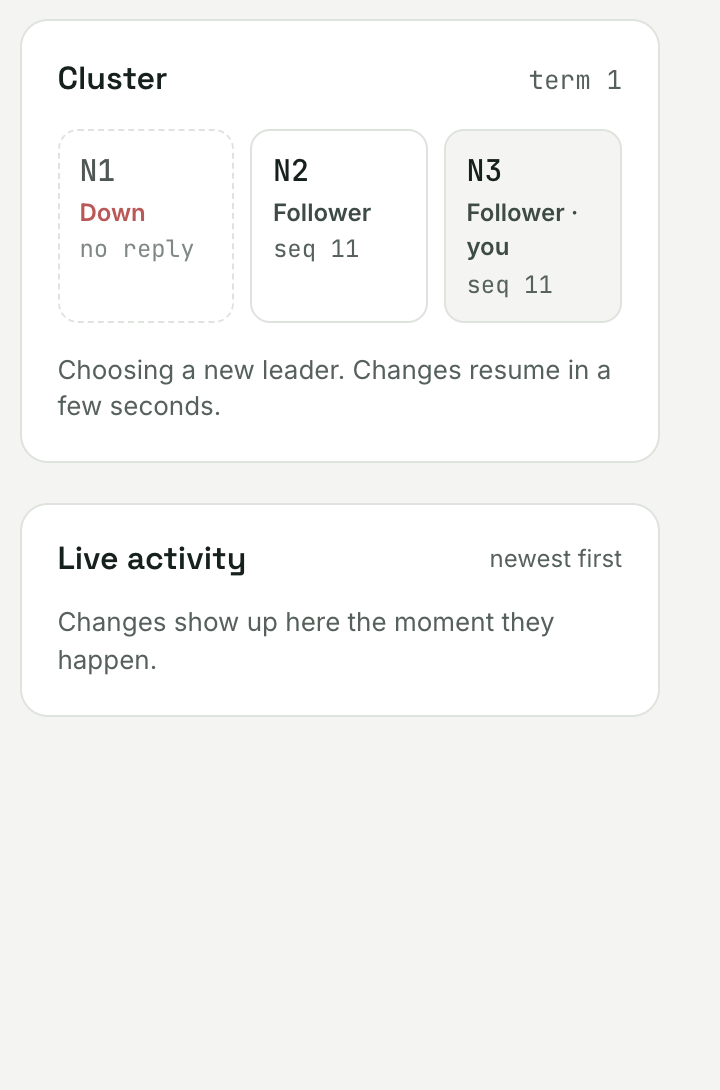
\includegraphics[width=0.24\textwidth]{failover-2-outage-cluster.png}\hfill
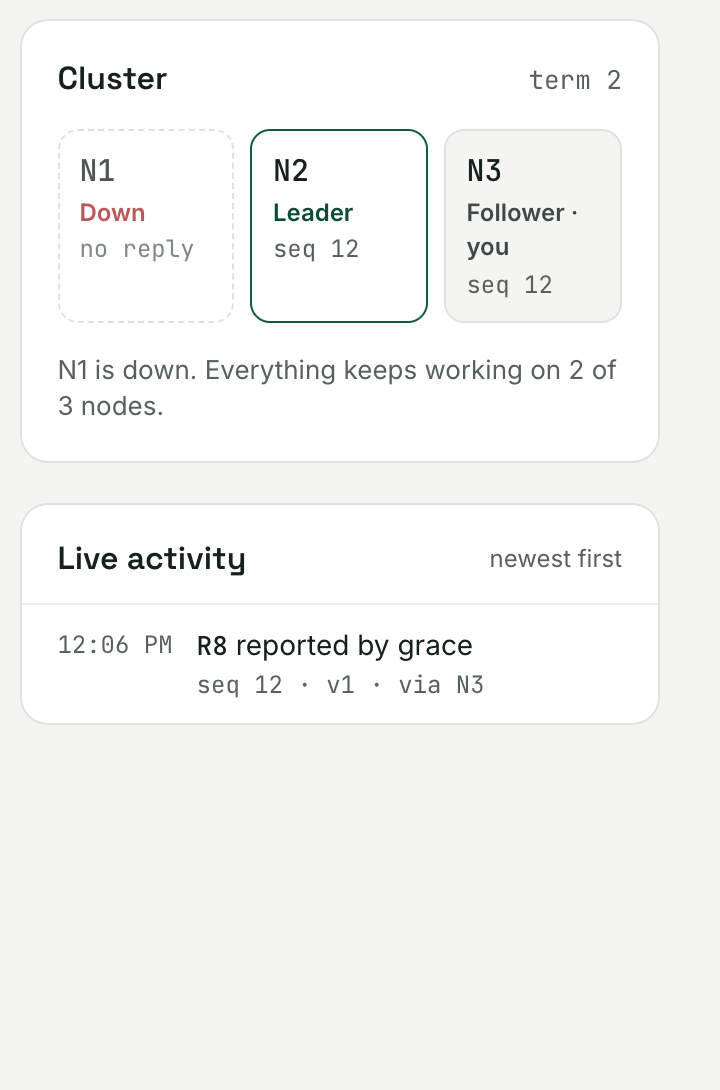
\includegraphics[width=0.24\textwidth]{failover-3-recovered-cluster.png}\hfill
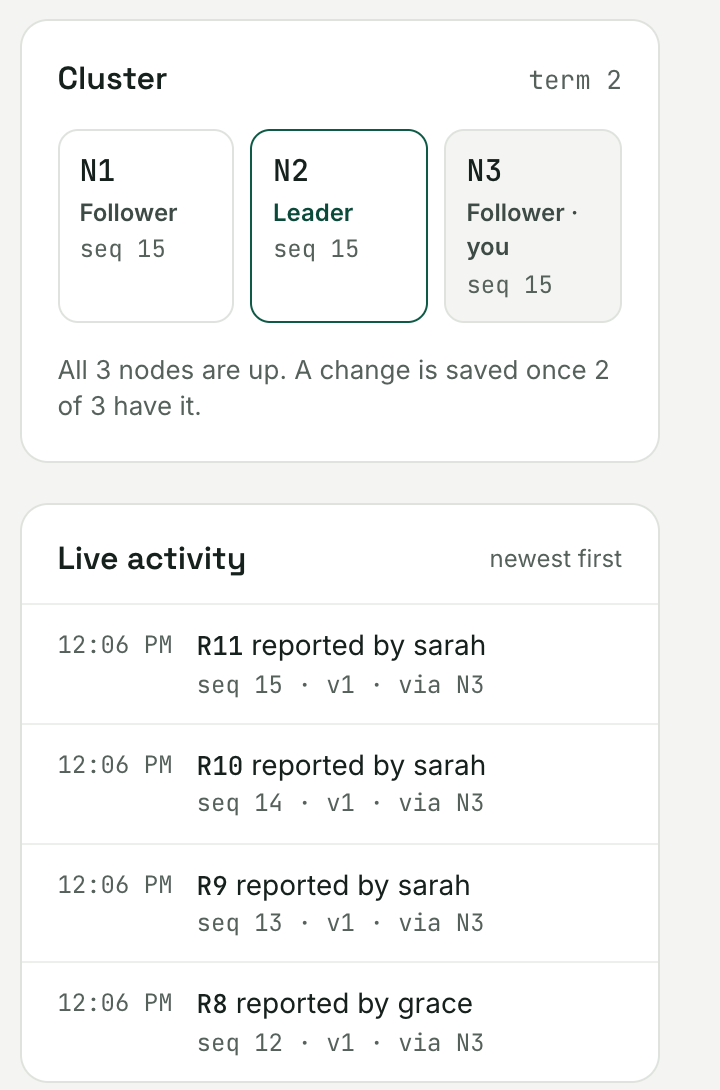
\includegraphics[width=0.24\textwidth]{failover-4-restarted-cluster.png}
\caption{The cluster panel of the web application during a leader failure, left to right.
(1) Before: N1 leads. (2) 1.5~s after N1 is killed: it shows as down and no leader exists yet;
reports can still be read. (3) 5.5~s after the kill: N2 leads in term~2 and the report submitted
during the outage (R8) has been saved. (4) N1 restarted: back as a follower with the same sequence
number as the others. Full-page screenshots are in \code{docs/img/}.}
\label{fig:browser}
\end{figure}

\subsection{Limits of the solution}

\begin{itemize}
\item \textbf{It tolerates the loss of one node of three.} With two down there is no majority
and writes fail with 503.
\item \textbf{Writes pause for about 3.3 seconds} when the leader fails. This is the 3~s
detection timeout plus the election. A single client may wait up to about 5~s because of its
retry schedule. A shorter timeout would recover faster but would mistake a
slow node for a dead one more often.
\item \textbf{Network partitions are only partly handled.} A leader cut off from the others
still believes it leads. It cannot reach a majority, so its writes fail with 503, but it has
already applied them locally, so reads from it may show changes that never committed. When the
partition heals, the higher term wins and the old leader resynchronises.
\item \textbf{The election is a simplification, not Raft or Paxos.} There is no voting and terms
are not stored on disk.
\item \textbf{There is no authentication.} Names and the moderator role are claimed by the
client.
\item \textbf{The log is never compacted,} so start-up replay time grows with history.
\end{itemize}

%======================================================================
\section{(e) Performance and scalability evaluation}
\label{sec:perf}

\subsection{Method}

Load tests ran against three real node processes on one laptop (8 CPU cores), measured on 10
November 2026. Each test case started a fresh cluster and ran $N$ concurrent clients for 15 seconds, for
$N = 10$, 50 and 100. Each client repeated a mix of operations: 60\% read one report, 10\%
filtered list, 15\% submit, 15\% update (a read followed by a PATCH). Updates targeted five
shared reports so that clients really collided. Clients were spread across all three nodes, so
forwarding from followers to the leader is included in the measurements. A 409 answer counts as
a success because it is the correct response to a stale edit.

\subsection{Results}

\begin{table}[H]
\centering
\begin{tabular}{@{}rrrrrrrrr@{}}
\toprule
Clients & Requests & Throughput & Avg & p95 & p99 & Success & 409 & Errors \\
 & & (req/s) & (ms) & (ms) & (ms) & rate & & \\
\midrule
10 & 70,236 & 4,681 & 2.1 & 9.6 & 17.1 & 100\% & 2.5\% & 0 \\
50 & 71,719 & 4,775 & 10.5 & 76.0 & 115.6 & 100\% & 3.5\% & 0 \\
100 & 64,711 & 4,302 & 23.1 & 186.9 & 261.8 & 100\% & 3.7\% & 0 \\
\bottomrule
\end{tabular}
\caption{Load test. After every run all three nodes held identical data and the WAL length
equalled the number of acknowledged writes.}
\end{table}

\begin{figure}[H]
\centering
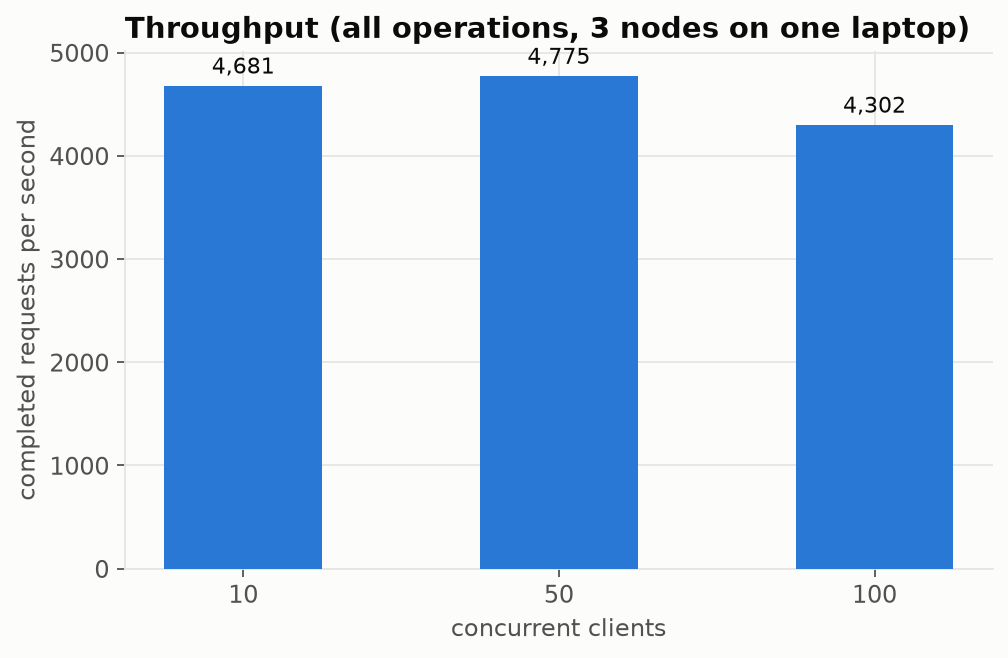
\includegraphics[width=0.49\textwidth]{load_throughput.png}\hfill
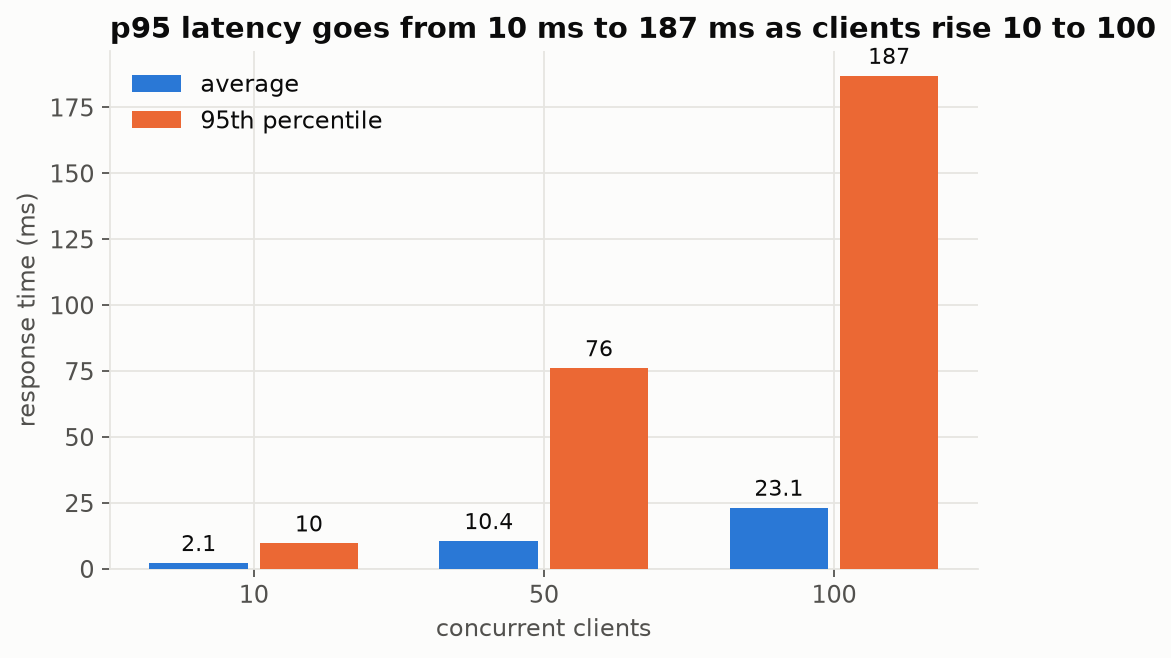
\includegraphics[width=0.49\textwidth]{load_latency.png}
\caption{Throughput (left) and response time (right) for 10, 50 and 100 clients.}
\end{figure}

\subsection{Interpretation}

\begin{itemize}
\item \textbf{Throughput is flat at about 4,300 to 4,800 requests per second.} Ten clients are
already enough to saturate the system; adding clients does not add capacity. At 100 clients
throughput falls by about 10\%, which is the cost of contention and thread switching.
\item \textbf{Response time grows roughly in proportion to the number of clients:} 2.1~ms,
10.5~ms and 23.1~ms on average. This is what a saturated system does: the same amount of work is
done per second, so each request spends longer waiting its turn.
\item \textbf{The slowest requests suffer most.} The 99th percentile rises from 17~ms to 262~ms.
These are mostly writes waiting behind other writes.
\item \textbf{Correctness holds under load.} The success rate stayed at 100\% with zero errors,
and the proportion of 409 answers rose only slightly (2.5\% to 3.7\%) as more clients collided on
the same reports.
\item \textbf{Submits are the bottleneck.} All submits share one lock (numbering and replication
happen inside it), whereas updates to different reports run in parallel. Batching several entries
into one replication request would be the first improvement.
\item \textbf{Recovery time is dominated by detection.} Of the 3.3~s outage, 3.0~s is the
dead-leader timeout; the election itself takes about 0.3~s. Restart recovery is fast (0.13~s for
about a thousand entries) because only the missing entries are transferred.
\end{itemize}

\paragraph{Cautions.} The load generator shared the laptop's CPU with the three nodes, so the
figures compare load levels with each other and are not the capacity of a real three-machine
deployment. Measuring also exposed a real fault: the first version opened a new TCP connection per
request and ran out of temporary ports under load; reusing connections (HTTP keep-alive with a
small pool) fixed it.

\subsection{Testing summary}

An automated suite of 46 tests covers the interface and WAL replay, concurrent edits,
replication, election and recovery, the live feed, and the features used by the web application.
All 46 pass; the log is in \code{results/test\_results.txt}.

%======================================================================
\section{Contributions}

\begin{description}[leftmargin=0cm,style=nextline]
\item[\memberA\ (cluster side)] Write-ahead log and store, the per-report locking design,
majority replication, heartbeats, terms and leader election, catch-up and resynchronisation, and
the failure benchmark. Report sections (a), (c) and (d).
\item[\memberB\ (client and interface side)] REST interface and status codes, client library
(timeout, retry, failover), command-line client, live feed and web application, and the load
benchmark. Report sections (b) and (e).
\end{description}
Both members wrote the tests for their own parts and present them in the demonstration.

%======================================================================
{document}
